\documentclass[xcolor=dvipsnames,table]{beamer}

\usepackage{latexsym}
\usepackage[utf8]{inputenc}
\usepackage[brazil]{babel}
\usepackage{amssymb}
\usepackage{amsmath}
\usepackage{stmaryrd}
\usepackage{fancybox}
\usepackage{datetime}
\usepackage[T1]{fontenc}
\usepackage{graphicx}
\usepackage{graphics}
\usepackage{url}
\usepackage{algorithmic}
\usepackage{algorithm}
\usepackage{acronym}
\usepackage{array}

\newtheorem{definicao}{Definio}
\newcommand{\tab}{\hspace*{2em}}

\mode<presentation>
{
  \definecolor{colortexto}{RGB}{0,0,0}
 
  \setbeamertemplate{background canvas}[vertical shading][ bottom=white!10,top=white!10]
  \setbeamercolor{normal text}{fg=colortexto} 

  \usetheme{Warsaw}
}

\title{Isomorfismo} 

\author{
  Esdras Lins Bispo Jr. \\ \url{bispojr@ufg.br}
  } 
 \institute{
  Teoria de Grafos \\Bacharelado em Ciência da Computação}
\date{\textbf{15 de agosto de 2017} }

\logo{
\includegraphics[width=1cm]{images/ufgJataiLogo.png}}

\begin{document}

	\begin{frame}
		\titlepage
	\end{frame}

	\AtBeginSection{
		\begin{frame}{Sumário}%[allowframebreaks]{Sumário}
    		\tableofcontents[currentsection]
    		%\tableofcontents[currentsection, hideothersubsections]
		\end{frame}
	}

	\begin{frame}{Plano de Aula}
		\tableofcontents
		%\tableofcontents[hideallsubsections]
	\end{frame}
    
   \begin{frame}{Pensamento}
   	\begin{columns}
   		\column{.4\textwidth}  		
   		\begin{center}
   			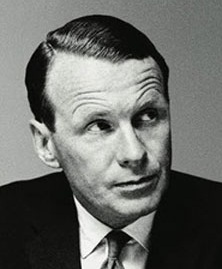
\includegraphics[height=.5\textheight]{images/ogilvy.jpg}
   		\end{center}
   		\column{.6\textwidth}  		
   		\begin{block}{Frase}
   			\begin{center}
   				{\large As normas existem para \\a obediência dos tolos e \\ para a orientação dos sábios.}
   			\end{center}
   		\end{block}		  		
   		\begin{block}{Quem?}
   			\begin{center}
   				{\bf David Ogilvy (1911-1999)} \\Publicitário inglês.
   			\end{center}
   		\end{block}
   	\end{columns}
   \end{frame}
    
    \section{Revisão}
	\subsection{Florestas e Árvores}
	\begin{frame}{Florestas e Árvores}
		\begin{block}{Floresta}
			\begin{itemize}
				\item Uma {\bf floresta} ($forest$) é um grafo sem circuitos.   
				\item Também chamado de grafo acíclico.   
				\item Um grafo é uma floresta se cada uma de suas arestas é uma ponte. 
			\end{itemize}
		\end{block}   
		\begin{block}{Árvore}
			Uma {\bf árvore} ($tree$) é uma floresta conexa. 
		\end{block}   
		\begin{block}{Corolário 1}
			Cada componente de uma floresta é uma árvore.
		\end{block}
	\end{frame}
	
	\begin{frame}{Florestas e Árvores}
		\begin{block}{Folha}
			Uma {\bf folha} ($leaf$) de uma floresta é qualquer vértice da floresta que tenha grau 1.
		\end{block}   
		\begin{block}{Corolário 2}
			Um grafo $G$ é uma floresta se e somente se $m(G) = n(G) - c(G)$.
		\end{block}
	\end{frame}
	
	\subsection{Planaridade}
	\begin{frame}{Grafos Planares}
		\begin{block}{Definição (informal)}
			Um grafo é {\bf planar} se pode ser desenhado no plano sem que as linhas que representam arestas se cruzem.
		\end{block}   
		\begin{block}{Exercícios}
			\begin{itemize}
				\item Todo caminho é planar? Todo circuito é planar?   
				\item Toda grade é planar?   
				\item Todo $K_4$ é planar? Todo $K_5$ é planar?   
				\item Todo $K_{2,3}$ é planar? Todo $K_{3,3}$ é planar?
			\end{itemize}
		\end{block}
	\end{frame}

	\section{Isomorfismo}
	\begin{frame}{Isomorfismo}
		\begin{block}{Definição}
			Um {\bf isomorfismo} entre dois grafos $G$ e $H$ é uma bijeção $f$ de $V(G)$ em $V(H)$ tal que dois vértices $v$ e $w$ são adjacentes em $G$ se e somente se $f(v)$ e $f(w)$ são adjacentes em $H$. Dois grafos são {\bf isomorfos} se existe um isomorfismo entre eles.
		\end{block}
		\pause
		\begin{block}{Problema}
			Dado dois grafos $G$ e $H$, verificar se existe um isomorfismo entre eles.
		\end{block}
		\pause
		\begin{block}{Solução}
			Basta examinar todas as bijeções de $V(G)$ e $V(H)$. Se cada um dos grafos tem $n$ vértices, esse algoritmo consome tempo proporcional a $n!$.
		\end{block}
	\end{frame}
	
	\begin{frame}{Isomorfismo}
		\begin{center}
			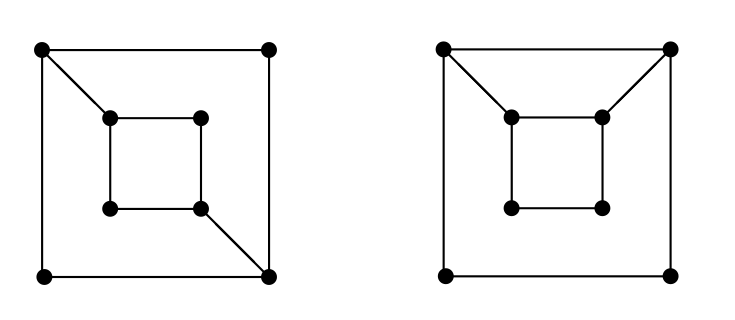
\includegraphics[width=8cm]{images/isomorfismo01.png}
		\end{center}
	\end{frame}
	
	\begin{frame}{Isomorfismo}
		\begin{center}
			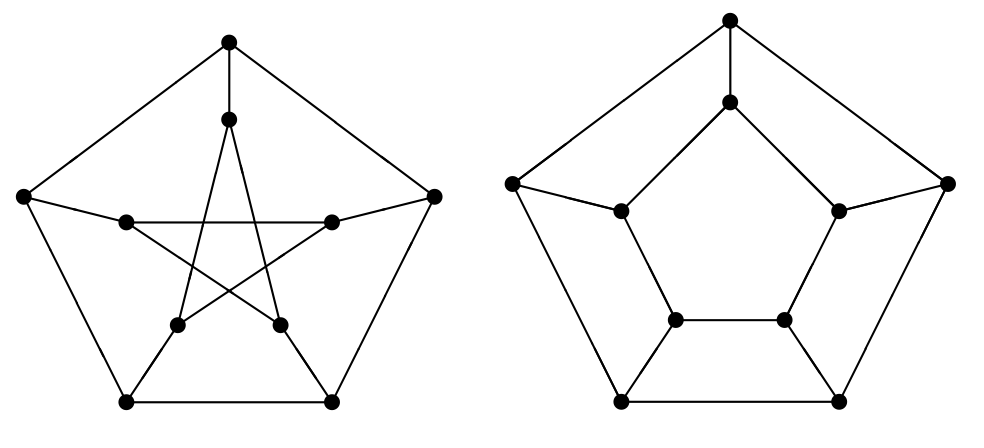
\includegraphics[width=8cm]{images/isomorfismo02.png}
		\end{center}
	\end{frame}
	
	\begin{frame}{Isomorfismo}
		\begin{center}
			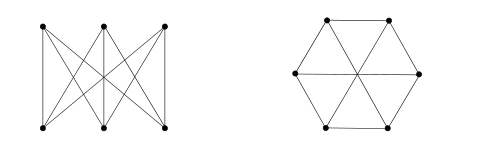
\includegraphics[width=10cm]{images/isomorfismo03.png}
		\end{center}
	\end{frame}
	
	\begin{frame}{Isomorfismo}
		\begin{block}{Corolário 01}
			Se $G$ e $H$ são isomorfos, então $|V(G)| = |V(H)|$.
		\end{block}
		\pause
		\begin{block}{Corolário 02}
			Se $G$ e $H$ são isomorfos, então $|A(G)| = |A(H)|$.
		\end{block}
		\pause
		\begin{block}{Corolário 03}
			Se $G$ e $H$ são isomorfos, então $\delta(G) = \delta(H)$ e $\Delta(G) = \Delta(H)$.
		\end{block}
	\end{frame}
	
	\begin{frame}
		\titlepage
	\end{frame}
	
\end{document}